\documentclass[a4paper,11pt,final]{report}
% Pour une impression recto verso, utilisez plutôt ce documentclass :
%\documentclass[a4paper,twoside,11pt,final]{article}

\usepackage[francais]{babel}
\usepackage[utf8]{inputenc}
\usepackage[T1]{fontenc}
\usepackage[pdftex]{graphicx}
\usepackage{setspace}
\usepackage[colorlinks=true,linkcolor=black,urlcolor=blue]{hyperref}
\usepackage[french]{varioref}
\usepackage[top=7em, bottom=7em, left=7em, right=7em]{geometry}
\usepackage{wrapfig}
\usepackage{fancyhdr}
\fancyhf{}
\renewcommand{\footrulewidth}{0.05em}
%entete
\lhead{\leftmark}
%pied depage
\cfoot{\thepage}
\lfoot{}
\rfoot{Desserte Robotisée}

\newcommand{\reporttitle}{Desserte Robotisée}     % Titre
\newcommand{\reportauthor}{Louis \textsc{LE CLEC'H}\\
                           Théophile \textsc{GUILBAUD}\\
                           Clément \textsc{BRISSET}}% Auteur
\newcommand{\reportsubject}{Environnement, démarche, et conception} % Sujet
\newcommand{\HRule}{\rule{\linewidth}{0.5mm}}
\newcommand{\siecle}[1]{\textsc{\romannumeral #1}ème}
\setlength{\parskip}{1ex} % Espace entre les paragraphes


\hypersetup{
    pdftitle={\reporttitle},%
    pdfauthor={\reportauthor},%
    pdfsubject={\reportsubject},%
   % pdfkeywords={rapport} {vos} {mots} {clés}
}

\begin{document}
  \begin{titlepage}
\begin{flushleft} 
  \large
  \emph{Auteur :}\\
  \reportauthor\\
\end{flushleft}
\begin{center}
  
  \begin{center}
    \begin{tabular}{c}
      \\
      
\includegraphics [width=60mm]{Images/ENSEIRB-MATMECA.jpg} \\
      \\
      
\includegraphics [width=70mm]{Images/logo-INRIA.jpg}\\
      \\
      \\
    \end{tabular}
    
    
      
    \textsc{\Large \reportsubject}\\[0.5cm]
           {\large 9 janvier au 28 janvier}\\
           
           
           \HRule \\[0.4cm]
                  {\huge \bfseries \reporttitle}\\[0.4cm]
                  \HRule \\[1.5cm]
                  
                  \begin{center}
                    
                    
                    
                    
                  
                  
                  %\vfill                  
                  
                  
                  
  \end{center}    
\end{center}
\begin{flushbottom}
\begin{flushright} 
  \large
  \emph{Responsables :} \\
  M.~David DANEY - \small{INRIA} \\
  M.~Christian MALAURIE - \small{Bordeaux 3}
\end{flushright}
\end{flushbottom}
\end{center}
\end{titlepage}

  %\cleardoublepage % Dans le cas du recto verso, ajoute une page blanche si besoin
  \tableofcontents % Table des matières
  \listoffigures
 % \sloppy          % Justification moins stricte : des mots ne dépasseront pas des paragraphes
  %\cleardoublepage
  \begin{onehalfspace}
  \pagestyle{fancy}

\chapter*{Introduction}
\addcontentsline{toc}{chapter}{Introduction}

%surement qu'il faudrait mettre le classique de la réalisation de tte introduction: accroche , problématique, analyse du devellopement du plan

\section{Comment concevoir dans un champ social}
%Ouaouh! on a construit des robots pour aller sur la lune mais le mettre avec des humains c'est plus difficile

L’industrie, la technique et la recherche sont déjà investies par les robots. Mais quand les considérerons-nous comme des partenaires à part entière de notre vie ? C’est à cette question que tend à répondre ce projet de desserte robotisée.

C’est à l’origine dans le domaine de l’industrie, notamment automobile, que les robots se sont d’abord et le plus durablement installés. Pour ensuite se trouver dans les zones nucléaires, les terrains minés, l’espace ou les abysses marins à très forte pression. Et c’est ainsi que le robot a su se faire une place dans ces milieux dit « extrêmes ». Mais il n’est pas encore très bien adapté au secteur du service.

Faire entrer un robot chez soi reste pour beaucoup un grand pas à franchir. Il faut donc réussir à faire rentrer le robot dans notre société de façon subtile. Alors l’acceptation du robot comme un atout pour l’être humain, et non comme un danger, deviendra possible.

A travers la desserte robotisée, nous offrons au robot une place de soutiens au service lors de cocktail. On l’intègre donc à une place de partenaire pour l’homme. Et c’est ainsi qu’il prend une place dans le champ humain sans s’y imposer de façon brusque.


\section{Le context du cocktail}

\subsection{Où se déroule un cocktail}
%lister les lieux

\subsection{Qui sont les acteurs du cocktail}
%lister les personnes

\subsection{Les ambiances d'un cocktail}
%lister les qualités

\subsection{Les complexités des niveaux d'intéractions dans le cocktail}
%lister les "`enjeux"' qui amènent les intéractions


\chapter{Spécification fonctionnelle}

\section{Les tâches principales}

\subsection{Se déplacer}

Le déplacement est bien entendu un élément cruciale de la conception
d'un robot. La desserte robotisée a ceci de particulier qu'elle doit
évoluer en milieu humain. Cela demande de définir exactement quand le
robot est en risque de rencontrer des humains, et comment il doit
réagir.

Au dela de cet aspect, nous devons également définir tous les types de
déplacements que le robot devra effectuer:

\begin{itemize}
\item Construction de carte
\item arrivée en salle
\item déambulation
\item gestion de groupe
\item suivi
\item dirigé
\item retour à la base
\item utilisation de l'interface
\end{itemize}

\subsubsection{Mode construction de carte}
La construction de carte est l'action primaire du robot lui permettant par la suite de se repérer dans la salle. C'est pourquoi elle doit se dérouler avant l'arrivée des convives ou après leur départ. C'est durant cette phase que le robot crée un carte de la salle de cocktail dans laquelle il va devoir se déplacer. Ainsi, lors de la réception, il pourra savoir se positionner dans la salle de réception.

La phase de construction de carte se déclenche par un élément externe comme le maître de réception. Pour déclencher se mode il faut que le robot soit dans la salle à cartographier. C'est à dire que le robot peut y être présent avant le lancement d'un autre mode de déplacement ou après avoir suivi la personne qui enclenchera le mode, soit après le mode suivi.

la cartographie se réalise à l'aide de deux caméra. Le robot se déplace seulement pour peaufiner sa carte. Sinon le robot tourne sur lui-même pour réaliser sa carte de repère. Ce mode se termine lorsque le robot a réalisé sa carte. 

Après avoir enclenché réalisé la carte, le robot devra rentrer à sa base avant le lancement de la soirée cocktail.

Les points d'entrées du mode sont:
\begin{itemize}
\item aucun mode
\item Le mode suivi
\end{itemize}

Les points de sorties du mode sont:
\begin{itemize}
\item le mode retour à la base.
\end{itemize}

\subsubsection{Mode arrivée en salle}

Le déplacement de la base vers la salle est la première chose que doit réaliser 
le robot avant de commencer sa déambulation. C’est donc  le moment où il vérifie 
que ses batteries sont chargées, que son plateau est rempli et qu’il connait le 
chemin vers la salle. Le mouvement de la base vers la salle peut être déjà cartographié.
Cet évènement ne peut arriver que s’il est déjà à sa base.

Les points d'entrées du mode sont:
\begin{itemize}
\item Le mode retour à la base
\item Le mode dirigé
\item Le mode suivi
\end{itemize}

Les points de sorties du mode sont:
\begin{itemize}
\item le mode déhambulation.
\end{itemize}


\subsubsection{Mode déambulation}

Le mode déambulation est l'un des princpaux mode de déplacement de la
desserte. Il s'agit pour le robot de repérer un groupe de convive puis
de se déplacer vers lui. Un des point clé de ce déplacement est que le
robot doit éviter de retourner sur une zone géographique qu'il à déjà
servi.

le déroulement du mode se fait comme suit:
\begin{itemize}
\item déclenchement du mode à l'arrivée dans la salle.
\item la disserte va de groupe en groupe et le cas échéant de table en
  table.
\item le robot garde en mémoire les zones géographiques déjà
  desservies et priorise les zones encore non servie.
\item Fin du mode de déambulation à la fin d'un timer et/ou après une
  diminution significative du poids du plateau, ou en cas d'absence
  d'espace ou passer (interieur d'un groupe), ou en cas de rencontre
  d'un groupe.\\
\end{itemize}

les points d'entrée du mode sont:
\begin{itemize}
\item le mode utilsation de l'interface
\item le mode arrivée en salle
\item le mode suivi
\item le mode dirigé\\
\end{itemize}

les points de sorties du mode sont:
\begin{itemize}
\item le mode suivi
\item le mode dirigé
\item le mode retour à la base
\item le mode gestion de groupe
\item le mode utilisation de l'interface\\
\end{itemize}

\subsubsection{Mode gestion de groupe}
Le mode de gestion de groupe est destiné au service d'un groupe de personnes. Suite à la prise de décision du robot de servir un groupe qu'il a détecté. Celui-ci rentre dans ce mode avant d'effectuer le service. Celui-ci commence par déterminer une hiérarchie dans le groupe lui permettant d'établir l'ordre le plus efficace et socialement correct pour servir les convives. La sortie du mode s'effectue une fois le service terminée.\\

Les points d'entrées du mode sont :
\begin{itemize}
\item mode déambulation
\end{itemize}

Les points de sortie du mode sont :
\begin{itemize}
\item mode déambulation
\end{itemize}

\subsubsection{Mode suivi}
Le mode suivi est un mode qui peut uniquement être activé et désactivé de façon manuelle via le mode utilisation interface.
Celui-ci est destiné à une utilisation exceptionnelle pour des cas spéciaux.

On pourra imaginer un mécanisme de sécurité implémenté dans l'interface qui permettra uniquement à des personnes habilitée d'activer ce mode de déplacement.
Une fois le mode activer, un émetteur amovible sera libéré et mis à la disposition de la personne ayant activer le mode.
Après activation du mode, le robot suivra cette émetteur en gardant une certain distance de sécurité, afin qu'en évitant tout se qui pourrait venir se placer dans son chemin. Cela permet donc d'emmenner le robot à n'importe quel endroit souhaité, par exemple une zone de chargement spéciale éloigné de la base du robot.\\


Les points d'entrées du mode sont :
\begin{itemize}
\item mode utilisation interface
\end{itemize}

Les points de sortie du mode sont :
\begin{itemize}
\item mode utilisation interface
\end{itemize}

\subsubsection{Mode dirigé}
Le mode dirigé permet au robot de faire des dessertes spéciales transmise par l'ordinateur centrale.
Cet ordre peut avoir été passé par le maitre d'hotel tout comme par un convive, demandant à un certain robot de changer de section, ou bien d'aller deservir une table ou un groupe particulier.
On peut aussi envisager de lui faire livrer une commande spéciale.\\

Le déroulement du mode se fait comme suit:
\begin{enumerate}
\item Commande reçue par l'ordinateur centrale
\item L'ordinateur centrale determine le meilleur robot pour effectuer la desserte
\item Si besoin, le robot choisie va à sa base pour récupérer ce dont il à besoin
\item Le robot effectue la desserte demandé\\
\end{enumerate}


Les points d'entrées du mode sont :
\begin{itemize}
\item mode déambulation
\item mode arrivée en salle
\item mode retour à la base
\end{itemize}

Les points de sortie du mode sont :
\begin{itemize}
\item mode déambulation
\item mode arrivée en salle
\item mode retour à la base
\end{itemize}

\subsubsection{Mode retour a la base}

Ce mode permet au robot de rentrer à la base lorsqu'il en a besoin
(ravitaillement, disfonctionnement, rappel du maitre d'hotel...).

le déroulement du mode se fait comme suit:
\begin{itemize}
\item déclenchement lorsque le plateau est vide et/ou timer, en cas de
  detection d'anomalie, ou de rappel à la base.
\item en cas de déplacement impossible, envoie une demande demande
  d'assistance.
\item cherche le plus court chemin ne passant pas par des groupes
\item fin du mode lorsque le robot arrive à la base.\\
\end{itemize}

les points d'entrée du mode sont:
\begin{itemize}
\item le mode déambulation
\item le mode utilsation de l'interface
\item le mode arrivée en salle
\item le mode suivi
\item le mode dirigé\\
\end{itemize}

les points de sorties du mode sont:
\begin{itemize}
\item le mode suivi
\item le mode dirigé
\item le mode utilisation de l'interface\\
\end{itemize}

\subsubsection{Mode utilisation interface}
Le robot entre dans ce mode lorsque quelqu'un utilise une des
interfaces du robot. Dans ce cas le robot doit cesser de se deplacer.

\subsection{schéma générale}

\begin{figure}[h]
\begin{center}
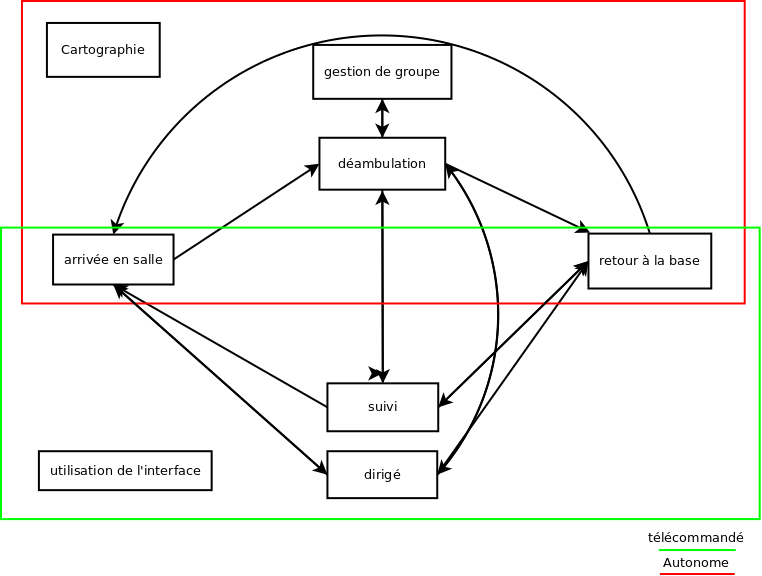
\includegraphics[scale=0.55]{Images/transition_mode.png}
\caption{Transition des modes}
\label{Transition des modes}
\end{center}
\end{figure}

\subsection{Servir}

\subsubsection{Maintenir le plateau}

\subsubsection{Presenter le plateau}

\subsection{Communication}
 


\section{Les tâches secondaires}

Les tâches principales du robot étant réalisé, il est toujours possible d’améliorer le robot en lui rajoutant des fonctionnalités pour réaliser des taches secondaires. C’est tâches ne seront pas détaillé par soucis de temps pour la réalisation de ce projet mais il serait intéressant d’y repenser. Pour vous aider dans vos réflexions, nous avons noté quelques idées.

\subsection{\^Etre un éléments d'échange entre les convives}

Le robot devrait pouvoir être un élément d’échange entre les convives. Il pourrait par exemple avoir des jeux sur lui ou des situations de rassemblement.

\subsubsection{Permettre à deux convives d'échanger discrètement}

Le robot pourrait être le messager discret entre deux convives.


\section{Caractéristiques}

\subsection{Communique}

\subsection{Se fait discret}


\chapter{Spécification techniques}

\section{Le Hardware}

\subsection{Le bras}

Pour assurer les mouvements de service et pour ranger le plateau lors
des déplacement un bras robotisé avec trois degrés de liberté est
suffisant pour reprendre les gestes d'un serveur, il devra cepandant
avoir comme caractéristique la possibilité de se retracter pour ranger
le plateau en position de déplacement.

Le plateau disposera également de capteur à ultrasons et/ou infrarouge
pour permettre de positionner le plateau aux bonnes distances par
rapport aux groupes ou aux personnes, soit un peu moins d'un mètre.
Cela implique cependant que le robot arrive à faire la différence entre 
une personne désirant se servir et une personne n'ayant pas vu le robot 
et ayant une trajectoire dangeureuse.

le plateau comme annoncé dans les contraintes liées au services a
traditionnellement un diamètre de $40cm$ que nous avons décidé de
conserver. Comme il doit être composé d'une matière disposant d'un
bonne isolation thermique, une base en acier inoxydable nous semble
être une solution cohérente.

Un capteur de pression devra être installé sur le plateau pour déterminer 
a quel moment le plateau doit être recharger.

\subsection{Le corps}

\subsubsection{Chassis}
Nous avons choisis de donner au robot un corps cylindrique d'un
diamètre légerement supérieur $45cm$. l'idée étant qu'en position de
déplacement, le plateau s'emboite légèrement dans le corps du robot.
La matière composant l'exterieur du chassis devras être relativement
souple pour minimiser un impact qui n'aurait pas pu être éviter. 

\subsubsection{Base mobile}
Pour ce qui est de la base mobile, nous avons choisi l'utilisation de
roue omnidirectionnelle, car les déplacements du robot demandent une
grande précision du fait de l'évolution en milieu humain, par contre
ce choix impose un sol totalement plat, ce qui exclut d'office tout
service en milieu exterieur.

\subsubsection{Sécurité}
Pour répondre aux contraintes de sécurités, nous nous somme inspirés
du robot numéro 1 (voir le chapitre sur l'état de l'art) et nous avons
choisis de coupler des capteur infrarouges à des capteurs à ultrasons
disposé tout autour du chassis pour permettre au robot d'éviter tout
contact. 

\subsubsection{Interface}
une surface tactile est prévue pour permettre à un utilisateur
d'interagir avec le robot (par exemple pour obtenir des information).

\subsubsection{autonomie}

\subsubsection{Caméra}

Outre les différents capteurs déjà cité pour le plateau ou la sécurité
du robot, une ou plusieurs caméras doit être installée sur le robot pour l'aider
d'une part à repérer des groupes de personnes, et d'autre part une
fois que le robot commence à servir le groupe, à éviter que le robot
aille servir trop de fois la même personne.

\subsubsection{}


\section{Le Software}


\section{design}


\end{onehalfspace}
\end{document}
